% \begin{savequote}[8cm]
% Alles Gescheite ist schon gedacht worden.\\
% Man muss nur versuchen, es noch einmal zu denken.

% All intelligent thoughts have already been thought;\\
% what is necessary is only to try to think them again.
%   \qauthor{--- Johann Wolfgang von Goethe \cite{von_goethe_wilhelm_1829}}
% \end{savequote}

\chapter{\label{ch:2-draft}Sample Chapter: Active Phase Separation}

\minitoc

\section{Introduction}

\section{Theory of Equilibrium Phase Separation}

\subsection{Free Energy}

\subsection{Phase Separation}

\subsection{}

\section{Catalysis Induced Phase Separation}

\subsection{Reaction Rates and Catalysis}

\subsection{Non-Interacting Phase Separation}

\section{\label{sec:intro}Introduction}
Aggregation and compartmentalisation within the cellular environment has been observed in a variety of contexts\cite{weber_drops_2021}. Droplet-like compartments can form reactors for certain cellular processes\cite{nott_phase_2015} or buffer noise in the cellular environment\cite{klosin_phase_2020} and aggregation of the $\alpha$-synuclein protein has strong links to the development of Parkinson's Disease\cite{tong_loss_2010}. Understanding the physical processes surrounding this phase separation and aggregation is nessecary to develop techniques to prevent or encourage this formation and may also identify further downstream consequences and effects.

A variety of both equilibrium and non-equilibrium mechanisms have been studied that can cause phase separation\cite{li_non-equilibrium_2020,weber_drops_2021}. Recently, the role chemical activity between the constituent components of a system have been explored and a rich phenomena beyond simple phase separation or aggregation can be observed \cite{agudo-canalejo_active_2019}. A potential limitation of these models may be their relevance to the exact values of system parameters which may not be found in the natural world. Conversely, enzymatic activity is ubiquitous and arguably necessary in living systems and an interesting question is whether this abundant activity can be a mechanism to cause such phase separation and aggregation.

\section{Building a Theoretical Model}
\subsection{\label{sec:rs_theory}Regular Solution Model}
A common description of two component fluid mixtures is the regular solution model \cite{jones2002soft}. This is a mean field model that describes a mixture of A molecules and B molecules on a lattice of N sites. The model consists of $n_A$ sites of molecule $A$ and $n_B=N_l-n_A$ sites of molecule $B$ which is described by a volume fraction $\phi_A = n_A/N_l$ and $\phi_B = n_B/N_l = 1-\phi_A$. The model identifies the free energy density of the system as (in units of $k_BT$)
\begin{equation}
    f_{RS} = \phi_A\ln\phi_A+\phi_B\ln\phi_B + \chi\phi_A\phi_B + \frac{K}{2}|\nabla\phi_A|^2
\end{equation}
where $\chi$ describes the interaction energy between the two components and the gradient term is related to a surface tension of the components. For a $\chi > 0$, there is an energetic cost to $A$ and $B$ occupying nearby sites and as such this drives the two components to separate. The model can be extended to a mixture of N-components and written in terms of the volume fractions, $\phi_i$, for each component

\begin{equation}
    f_{RS} = \sum_{i=1}^{N}\Bigg[\phi_i\ln\phi_i+\sum_{j=1, j\neq i}^{N}\frac{\chi_{ij}}{2}\phi_i\phi_j + \sum_{j=1}^{N} \frac{K_{ij}}{2}(\nabla\phi_i)\cdot(\nabla\phi_j)\Bigg]
    \label{rsm_gen}
\end{equation}

where the scalars $\chi$ and $K$ now become $N \times N$ matrices describing the interactions between components and the surface tensions between domains of different compositions \cite{berry_physical_2018}. The constant number of lattice sites, $N_l$ naturally imposes incompressibility into the model ensuring that $\sum_{i=1}^N\phi_i=1$.

\subsection{\label{sec:multi_fh}Generalised Model}
The Flory-Huggins model provides an extension to this regular solution model to reflect the different components as being molecules of different sizes. The model originally described polymers of chain length $N_P$ and introduced a correction to the entropic terms since the monomers on the chain are attached to each other which reduces the number of available configurations. We use this principle generally to extend the regular solution model in equation (\ref{rsm_gen}) to describe components of different size. This gives
\begin{equation}
    f_{FH} = \sum_{i=1}^{N}\Bigg[\frac{\phi_i}{v_i}\ln\phi_i+\sum_{j=1, j\neq i}^{N}\frac{\chi_{ij}}{2}\phi_i\phi_j + \sum_{j=1}^{N} \frac{K_{ij}}{2}(\nabla\phi_i)\cdot(\nabla\phi_j)\Bigg]
    \label{fh_gen}
\end{equation}
where $v_i$ describes the relative volumes of the components in the mixture. 

Another important contribution is from the intrinsic energy, the enthalpy, of each type of molecule which will appear proportionally to the number of molecules of that component in the system, $e_i \phi_i / v_i$. Previous work has often ignored this contribution as in a system of constant overall composition this term is simply an additive constant and so does not affect the behaviour of the solution. However the composition of a chemically active system can change and therefore this contribution may affect the system's behaviour.

The phase behaviour of these regular solution models is often dominated by the value of the interaction parameter, $\chi$. For $\chi > 0 $, there is an energetic cost to having different components mixing and can lead to phase separation. The interplay of entropic effects driving a homogeneous mixed state balanced against these additional terms determines the phase transitions. However all of these terms are derived from a free energy and provide an equilibrium description of the system. In fact, additional terms can be added to this equilibrium free energy density, such as terms from a generic external potential or higher order gradient terms. This project aims to explore the role of activity in these mixtures and as such we set $\chi = 0$, $K = 0$ and ignore all other interaction effects, so that the consequences of the activity are more obvious. It is understood that reintroducing these terms, for example a non-zero $\chi$, will simply make it harder/easier for these active effects to drive phase separation. This results in the free energy density
\begin{equation}
    f = \sum_{i=1}^{N}\frac{1}{v_i}\Bigg[e_i\phi_i + \phi_i\ln\phi_i\Bigg].
    \label{f}
\end{equation}

\section{Dynamics of Active Mixtures}

\subsection{Model B}
Model B dynamics can be used to describe the dynamical approach of a system to equilibrium \cite{li_non-equilibrium_2020}. The model describes the evolution of conserved quantities which describe the response of the volume fractions to the free energy. The model B dynamics are given by \cite{cates_active_2019}
\begin{equation}
    \dot{\phi}_i = - \nabla \cdot \textbf{J}_i
    \label{modB1}
\end{equation}
where $i$ runs across the components in the mixture, with $\textbf{J}_i$ given by
\begin{equation}
    \textbf{J}_i = \sum_j M_{ij}\nabla\mu_j + \textbf{J}^N
    \label{modB2}
\end{equation}
and where $\textbf{J}^N$ describes the noise, obeying the appropriate fluctuation dissipation theorems. Here, we consider the thermodynamic limit of a noise free model and set the $ \textbf{J}^N$ contribution to zero. The chemical potential for each component, $\mu_i$, is given by
\begin{equation}
    \mu_i = \frac{\delta F}{\delta \phi_i}
\end{equation}
which we can find directly for a non interacting system described by equation (\ref{f}) to be
\begin{equation}
    \mu_i = e_i + \log\phi_i + 1 \quad \text{and so} \quad \nabla\mu_i = \frac{1}{\phi_i}\nabla\phi_i.
    \label{chempots}
\end{equation}

\subsection{Active Dynamics}

\subsubsection{Thermodynamics of Chemical Reactions}
The model described so far considers only equilbirium terms and can be entirely described by a free energy. Here, we want to study the effect of non-equilibrium chemical activity in mixtures. Consider an isolated reaction that converts between two species, $A \rightleftharpoons B$. An immediate consequence of this reaction for an incompressible mixture is that the volume of a $A$ and $B$ must be equal. In general the volume of the reactants must equal the volume of the products which is simple for this 1:1 stoichiometry but could be more complex for non-conserved particle number.

The total number $A$ and $B$ particles in the system is constant, which allows us to define as $\alpha \equiv \phi_A+\phi_B$. Considering detailed balance for the system constrains the relationship between the forward and backward reaction rates
\begin{equation}
    \frac{r_{A \rightarrow B}}{r_{B \rightarrow A}} = \exp\Bigg(\frac{\mu_A - \mu_B}{k_B T}\Bigg)
    \label{db_constr}
\end{equation}
which allows us to identify the net transfer from $A \rightarrow B$ as
\begin{equation}
    r_{A \rightarrow B} - r_{B \rightarrow A} = K\Bigg(\exp\bigg(\frac{\mu_A - \mu_B}{k_B T}\bigg)-1\Bigg)
    \label{react_rates}
\end{equation}
which makes sense as if $\mu_A > \mu_B$ then we have net $A \rightarrow B$, when $\mu_B > \mu_A$ then we have net $B \rightarrow A$ and at equilibrium $\mu_A = \mu_B$\cite{weber2019physics}.

\subsubsection{Enzymatic Activity}
Enzymes act as catalysts in biological reactions and increase the rate of a reaction. This can be achieved by the presence of an active site that allows the reaction to occur with a lower activation energy, however here we model a fuel driven reaction that occurs only in the presence of this \textit{enzyme} component. The reaction that now occurs is
\begin{equation}
    \text{Fuel} + A \rightarrow \text{Waste} + B
\end{equation}
where the system is in contact with a Fuel and Waste reservoir that maintains constant chemical potentials, $\mu_{Fuel}$ and $\mu_{Waste}$ and we define $\Delta\mu \equiv \mu_{Fuel}-\mu_{Waste}$ which is also constant. Using equation (\ref{db_constr}) the rate of $A \rightarrow B$ of this reaction in the presence of the enzyme can be written as
\begin{equation}
    r_{A \rightarrow B,E} - r_{B \rightarrow A,E} = K'\phi_E\Bigg(\exp\bigg(\frac{\mu_A - \mu_B + \Delta\mu}{k_B T}\bigg)-1\Bigg)
    \label{enz_rates}
\end{equation}
where the reaction rate is proportional to the volume fraction of the enzyme component ($\phi_E$) and as such the constants $K$ and $K'$ (in equations (\ref{react_rates}) and (\ref{enz_rates}) respectively) have different units. Often this rate is described using Michaelis–Menten kinetics, which has a more complex form \cite{murray_mathematical_1993}. However to first order in a dilute enzyme system, the rate grows linearly with the volume fraction of enzyme and so we expect this description is able to encapsulate the key behaviour.

\subsection{\label{sec:min_mix}Minimal Active Mixture}

The most simple model that will encapsulate all of these effects requires at least two components for a chemical reaction to occur, e.g. $S \rightleftharpoons P$ (substrate to product) and a third enzyme component (E), that permits the driven, catalytic reaction described in equation (\ref{enz_rates}). The system is therefore described by three volume fractions; $\phi_S$, $\phi_P$ and $\phi_E$. We study incompressible mixtures and so $\phi_S+\phi_P+\phi_E=1$ (giving $\alpha=1-\phi_E$) and this also requires the volume of the substrate and product be the same, $v_S=v_P$. In real catalytic systems, the enzyme is often larger than the substrate and product ad so we expect $v_E > v_S, v_P$\cite{berg_biochemistry_2002}. This increased size is also expected to result in increased damping and the enzyme moving slower through a fluid in response to a potential.

In this three component model, all components evolve in response to the Model B dynamics via the mobilities and gradients in chemical potential. Additionally, the substrate and product evolve as a consequence of reactions. This gives
\begin{align}
    \dot{\phi}_E &= \nabla \cdot \big(M_{EE}\nabla\mu_E + M_{ES}\nabla\mu_S + M_{EP}\nabla\mu_P) \label{evoE}\\
    \dot{\phi}_S &= \nabla \cdot \big(M_{SE}\nabla\mu_E + M_{SS}\nabla\mu_S + M_{SP}\nabla\mu_P) - R \label{evoS}\\
    \dot{\phi}_P &= \nabla \cdot \big(M_{PE}\nabla\mu_E + M_{PS}\nabla\mu_S + M_{PP}\nabla\mu_P) + R \label{evoP}
\end{align}
where the contribution from chemical reactions is described by $R = r_{spo} + r_{cat}$, the contribution from the spontaneous reaction and from the catalysed reaction (note that these contributions might be negative as this flux is always expressed in the direction $S \rightarrow P$). The reaction contributions are described using equations (\ref{react_rates}) and (\ref{enz_rates}) to give
\begin{align}
    r_{spo} &= K_{spo}[\text{exp}(\mu_S-\mu_P) - 1] = k_{spo}[e^{\Delta e}\phi_S - \phi_P] \\
    r_{cat} &= K_{cat}\phi_E[\text{exp}(\mu_S - \mu_P + \Delta\mu) - 1] = k_{cat}\phi_E[\phi_S-\phi_P e^{-(\Delta e+ \Delta\mu)}]
\end{align}
where the chemical potential given in equation (\ref{chempots}) is used and $\Delta e = e_S - e_P$. The rate constants here have been scaled to better disentangle the effects of the various parameters; $k_{spo} = K_{spo}/\phi_P$ and $k_{cat} = K_{cat}e^{-(\Delta e + \Delta \mu)}/\phi_P$.

\section{Choices for Mobilities}
\subsection{Incompressible Fluids}

Model B dynamics for a system introduce mobilities, $M_{ij}$ which describe how the $i^{\text{th}}$ component responds to the $j^{\text{th}}$ chemical potential. Prior work has investigated similar quantities, $\widetilde{M}_{ij}$ which describe the responses of the concentrations of components $c_j$ with $c_j = \frac{\phi_j}{v_j}$. $\widetilde{M}_{ij}$ has been shown to be symmetric $\widetilde{M}_{ij} = \widetilde{M}_{ji}$ and positive semi-definite $\widetilde{M}_{ij} \succcurlyeq 0$\cite{onsager_reciprocal_1931}. These concentration mobilities can be related to the volume fraction mobilities by a factor of the volume ${M}_{ij} = v_i\widetilde{M}_{ij}$, or as a matrix equation $M = \text{diag}[v_1, .., v_N]\cdot\widetilde{M}$, and this gives
\begin{equation}
    {M}_{ij} = \frac{v_i}{v_j}{M}_{ji}.
    \label{mobsym}
\end{equation}

The incompressibility condition can be written as $\sum_i\phi_i = 1$ and so $\sum_i\dot{\phi}_i = 0$. Equations (\ref{modB1}) and (\ref{modB2}) allow this relation to be expanded in the noise free model
\begin{equation}
    \sum_i\dot{\phi}_i = \sum_i\;\nabla\cdot\bigg(\sum_j M_{ij}\nabla\mu_j\bigg) = \sum_j\;\nabla\cdot\bigg(\big(\sum_i M_{ij}\big)\nabla\mu_j\bigg) = 0
\end{equation}
In order for this to be true in general, for non-uniform systems, i.e. $\nabla\mu_j \neq 0$, it is necessary for the mobilities to satisfy
\begin{equation}
    \sum_i M_{ij} = 0
    \label{mobinc}
\end{equation}
which constrains the mobilities and enforces the fluid remains incompressible. For an $N$-component mixture, the self- and cross-mobilities can be described in an $N\times N$ matrix. Equation (\ref{mobinc}) reduces the number of free parameters to $N(N+1)/2$ for a generic system and when the incompressibility condition is also included, equation (\ref{mobinc}), this is further reduced to $N(N-1)/2$ free parameters. There is also the constraint from the reciprocal relations, that $\widetilde{M} = \text{diag}[v_1, .., v_N]^{-1}M \succcurlyeq 0$.

The choice of these free variables is often described by Kramer's form\cite{KRAMER1984473}, that the mobility is $M_{ij}$ is proportional to the volume fractions $\phi_i$ and $\phi_j$. A common choice is to assume $M_{ij} = D(\delta_{ij}\phi_i - \phi_i\phi_j)$ which imposes the necessary  symmetry and incompressibility constraints for components of equal sizes (same $v_i$ for all components). The prefactor diffusion constant, $D$, also indicates that the fluxes of each component are similar in response to potentials, but as discussed, we expect particles of different sizes to respond in different ways. Instead, a more general scheme is to assume that $M_{ij} = -D_{ij}\phi_i\phi_j$ for $i \neq j$ and then $M_{ii}$ is constructed such that the incompressibility condition is satisfied (equation (\ref{mobinc})).


\subsection{Mobilities for E, S, P}
As an example we consider the three component (E, S, P), minimal active mixture. Due to the incompressibility condition, we have $v_S=v_P$ and so we can write the mobility matrix as
\begin{equation}
M = 
\begin{pmatrix}
M_{EE} & M_{ES} & M_{EP}\\
M_{SE} & M_{SS} & M_{SP}\\
M_{PE} & M_{PS} & M_{PP}\\
\end{pmatrix}
=
\begin{pmatrix}
-(M_{SE}+M_{PE}) & M_{SE}\frac{v_E}{v_S} & M_{PE}\frac{v_E}{v_P}\\
M_{SE} & -(M_{SE}\frac{v_E}{v_S}+M_{SP}) & M_{SP}\\
M_{PE} & M_{SP} & -(M_{PE}\frac{v_E}{v_P}+M_{SP})\\
\end{pmatrix}
\label{ESP_mob}
\end{equation}
The free mobilities to be defined here are $M_{SE}$, $M_{PE}$, and $M_{SP}$, which in general can be a function of $\phi_E$, $\phi_S$, and $\phi_P$.

\section{Stability of the Homogeneous Steady State}
\subsection{Minimal Active Mixture}
The minimal active mixture described by equations (\ref{evoE})-(\ref{evoP}) can be seen to have a uniform steady state solution when $R=0$. All other terms describing the evolution from gradients in the chemical potentials vanish for a homogeneous system and solving for $R=0$ yields the stationary state with
\begin{align}
    \phi_S^* = \alpha\frac{(k_{cat}\phi_E^*-k_{spo})}{k_{cat}\phi_E^*(e^{\Delta e + \Delta\mu}+1) - k_{spo}(\text{exp} (\Delta e)+1)} \label{sstar}
    \\
    \phi_P^* = \alpha\frac{(k_{cat}\phi_E^*\text{exp} (\Delta e + \Delta\mu) - k_{spo}(\text{exp} (\Delta e))}{k_{cat}\phi_E^*(\text{exp} (\Delta e + \Delta\mu)+1) - k_{spo}\text{exp} (\Delta e+1)} 
    \label{pstar}
\end{align}
where the star indicates that these quantities are at $R=0$ and $\alpha$ is the total amount of product and substrate in the system $\alpha = \phi_S^*+\phi_P^*$ and for the minimal mixture case, $\alpha = 1-\phi_E^*$. We consider a small perturbation from this uniform steady state $\phi_i \rightarrow \phi_i^* + \delta\phi_i$ giving $\mu_i \rightarrow \mu_i^* + \delta\mu_i$. Equation (\ref{chempots}) gives $\delta\mu = \frac{\delta\phi_i}{\phi_i^*}$ and so $\nabla\mu_i = \frac{1}{\phi_i^*}\nabla\delta\phi_i$ (both to first order) and also define $M^*_{ij} = M_{ij}(\phi_E^*, \phi_S^*, \phi_P^*)$. Finally, expand $R$ around the $R=0$ solution, to give $\delta R = R_E\delta\phi_E+R_S\delta\phi_S-R_P\delta\phi_P$ (where the signs are chosen such that all $R_i \geq 0$).
\begin{align}
    R_E &= k_{cat}[\phi_S^*-\phi_P^*e^{(\Delta e + \Delta \mu)}] = \alpha\frac{k_{cat}k_{spo}(1-e^{\Delta \mu})}{k_{spo}+k_{cat}\phi_E^*e^{-(\Delta e + \Delta \mu)}+k_{spo}e^{\Delta e}+k_{cat}\phi_E^*}\\
    R_S &= k_{spo}e^{\Delta e} + k_{cat}\phi_E^*\\
    R_P &= k_{spo} + k_{cat}\phi_E^*e^{-(\Delta e+\Delta \mu)}
\end{align}

We consider perturbations from this steady state of the form $\delta\phi_i = |\delta\phi_i| e^{i\textbf{q}\cdot\textbf{r}}$ and the resulting linear response of the system can be written as

\noindent
\makebox[\textwidth]{\parbox{1.3\textwidth}{%
\begin{equation}
\begin{pmatrix}
\dot{\delta\phi_E}\\
\dot{\delta\phi_S}\\
\dot{\delta\phi_P}\\
\end{pmatrix} =
\underbrace{
\begin{pmatrix}
(M_{SE}^*+M_{PE}^*)\frac{\textbf{q}^2}{\phi_E^*} & -M_{SE}^*\frac{v_E}{v_S}\frac{\textbf{q}^2}{\phi_S^*} & -M_{PE}^*\frac{v_E}{v_P}\frac{\textbf{q}^2}{\phi_P^*}\\
-M_{SE}^*\frac{\textbf{q}^2}{\phi_E^*} - R_E & \big(M_{SP}^* + M_{SE}^*\frac{v_E}{v_S}\big)\frac{\textbf{q}^2}{\phi_S^*} - R_S & -M_{SP}^*\frac{\textbf{q}^2}{\phi_P^*} + R_P\\
-M_{PE}^*\frac{\textbf{q}^2}{\phi_E^*}  + R_E & -M_{SP}^*\frac{\textbf{q}^2}{\phi_S^*} + R_S & \big(M_{PE}^*\frac{v_E}{v_P}+M_{SP}^*\big)\frac{\textbf{q}^2}{\phi_P^*} - R_P\\
\end{pmatrix}
}_{C}
\begin{pmatrix}
\delta\phi_E\\
\delta\phi_S\\
\delta\phi_P\\
\end{pmatrix}
\end{equation}}}
where we can explicitly see the incompressibility being imposed as the columns of $C$ sum to zero
\begin{equation}
    \sum_i\dot{\delta\phi_i} = \sum_{i,j}C_{ij}\delta\phi_j = \sum_{j}0\times\delta\phi_j = 0
\end{equation}
which allows one of the components to be eliminated. As an example, set $\delta\phi_P = -\delta\phi_E - \delta\phi_S$ and thus we can define a $2\times2$ matrix, $C'$ describing the evolution where we subtract the last column of the other two, i.e. $C'_{ij} = C_{ij} - C_{i3}$ for $i, j \in {1, 2}$, giving
\noindent
\makebox[\textwidth]{\parbox{1.3\textwidth}{%
\begin{equation}
\begin{pmatrix}
\dot{\delta\phi_E}\\
\dot{\delta\phi_S}\\
\end{pmatrix} =
\underbrace{
\begin{pmatrix}
(M_{SE}^*+M_{PE}^*)\frac{\textbf{q}^2}{\phi_E^*} +M_{PE}^*\frac{v_E}{v_P}\frac{\textbf{q}^2}{\phi_P^*}& -M_{SE}^*\frac{v_E}{v_S}\frac{\textbf{q}^2}{\phi_S^*} + M_{PE}^*\frac{v_E}{v_P}\frac{\textbf{q}^2}{\phi_P^*}\\
-M_{SE}^*\frac{\textbf{q}^2}{\phi_E^*} - R_E + M_{SP}^*\frac{\textbf{q}^2}{\phi_P^*} - R_P & \big(M_{SP}^* + M_{SE}^*\frac{v_E}{v_S}\big)\frac{\textbf{q}^2}{\phi_S^*} - R_S + M_{SP}^*\frac{\textbf{q}^2}{\phi_P^*} - R_P\\
\end{pmatrix}
}_{C'}
\begin{pmatrix}
\delta\phi_E\\
\delta\phi_S\\
\end{pmatrix}
\end{equation}}}
The eigenvalues of $C'$ determine the stability of the steady state. The system is stable if and only if all of $C'$'s eigenvalues are negative. Since $C'_{1,1}$ and $C'_{2,2}$ are always negative (from the Onsager constraints and the non-negativity of $R_i$), $\text{tr}(C') < 0$ and there is therefore one positive eigenvalue if $\det(C')<0$. The instability condition then becomes
\begin{equation}
\begin{split}
    \Bigg((M_{SE}^*+M_{PE}^*)&\frac{\textbf{q}^2}{\phi_E^*} + M_{PE}^*\frac{v_E}{v_P}\frac{\textbf{q}^2}{\phi_P^*}\Bigg)\Bigg(\big(M_{SP}^* + M_{SE}^*\frac{v_E}{v_S}\big)\frac{\textbf{q}^2}{\phi_S^*} - R_S + M_{SP}^*\frac{\textbf{q}^2}{\phi_P^*} - R_P\Bigg) \\
    &< \Bigg(-M_{SE}^*\frac{v_E}{v_S}\frac{\textbf{q}^2}{\phi_S^*} + M_{PE}^*\frac{v_E}{v_P}\frac{\textbf{q}^2}{\phi_P^*}\Bigg)\Bigg(-M_{SE}^*\frac{\textbf{q}^2}{\phi_E^*} - R_E + M_{SP}^*\frac{\textbf{q}^2}{\phi_P^*} - R_P\Bigg)
\end{split}
\label{hi_ord_ins}
\end{equation}
For very large values of $\textbf{q}$, we expect the system to be stable as in this regime the evolution is dominated by diffusive effects. When $\textbf{q} \rightarrow 0$ the system should be at the critical stability as this corresponds to a uniform change in the $\phi_i$s. As such, since this condition only depends on $\textbf{q}^2$ and $\textbf{q}^4$ the instability is satisfied if and only if it is satisfied for very small $\textbf{q}^2$. With this is mind we take equation (\ref{hi_ord_ins}) to first order in $\textbf{q}^2$ which gives
\begin{align}
    \frac{1}{v_E\phi_E^*}+\frac{1}{v_P(1-\phi_E^*)} < \frac{R_E}{v_P(1-\phi_E^*)}\bigg(\frac{\gamma_P}{R_S}-\frac{\gamma_S}{R_P}\bigg)
    \label{eq_form_cond}
\end{align}
where we have defined
\begin{equation}
    \gamma_S \equiv \frac{M_{SE}^*}{M_{SE}^*+M_{PE}^*} \quad \text{   and    } \quad \gamma_P \equiv \frac{M_{PE}^*}{M_{SE}^*+M_{PE}^*}
\end{equation}
Remembering that $R_E \propto (e^{\Delta\mu} - 1)$ we see that for $\Delta\mu=0$, $R_E = 0$ and the instability cannot be satisfied at equilibrium. This condition can also be written to constrain the relative volumes in the system
\begin{equation}
    \frac{v_P}{v_E} < \frac{\phi_E^*}{1-\phi_E^*}\Bigg(R_E\bigg(\frac{\gamma_P}{R_S}-\frac{\gamma_S}{R_P}\bigg) - 1\Bigg)
    \label{vol_ins}
\end{equation}
We can assume a form for $M_{SE} = -D_{SE}\phi_E\phi_S$ and $M_{PE} = -D_{PE}\phi_E\phi_P$ which results in
\begin{equation}
    \frac{1}{v_E\phi_E^*}+\frac{1}{v_P(1-\phi_E^*)} < \frac{R_E}{v_P(1-\phi_E^*)}\frac{D_{PE}-D_{SE}}{D_{PE}R_S+D_{SE}R_P}
\end{equation}
\begin{equation}
\begin{split}
\text{RHS} &= \frac{k_{cat}k_{spo}(1-e^{-\Delta\mu})}{v_P(k_{spo}+k_{cat}\phi_E^*e^{-(\Delta e+\Delta\mu)}+k_{spo}e^{\Delta e}+k_{cat}\phi_E^*)} \\ 
& \quad \quad \times \frac{D_{PE}-D_{SE}}{D_{PE}(k_{spo}e^{\Delta e}+k_{cat}\phi_E^*)+D_{SE}(k_{spo}+k_{cat}\phi_E^*e^{-(\Delta e+\Delta\mu)})}
\end{split}
\end{equation}
In calculating this condition we eliminated the product component from the system and determined the stability from considering the other two components. Alternatively, we could have eliminated either of the other components and require the same negative eigenvalues stability condition, which give the same result. A quick check for eliminating the substrate instead can be seen by noticing the expression is invariant under $S, P \rightarrow P, S$ and $R_E \rightarrow -R_E$, which is the same difference between the second and third rows of $C'$. Prior work often imposes incompressibility by eliminating one of the components and using $\phi_i = 1-\sum_{j,j\neqi}\phi_j$. This can be an effective equilibrium description, but when the approach to equilibrium and dynamics and considered, the correct choices for mobilities must also be constructed to impose the incompressibility naturally.

Larger $D_{PE}-D_{SE}$ makes the system more unstable. This can be understood, as $D_{PE}$ is a measure of how quickly the product component moves to regions of higher enzyme concentration. Since the enzyme allows for more product, this creates a feedback where the product moves to product faster than the substrate and this makes the system unstable. This preferential attraction must overcome the diffusive behaviour of the system to drive the instability. Equation (\ref{vol_ins}) also shows the stability depends on the ratio of $\frac{v_S}{v_E}$. The system is more unstable for much larger enzyme sizes compared to the substrate and product which is a convenient result since, as previously discussed, enzymes are often significantly larger than the substrate or products involved in the corresponding reaction. A similar size dependence can be seen in colloidal systems. Depletion forces arise from a particle of  intermediate size (between the size of the solvent and colloids) having an increased available volume to occupy when the colloids aggregate, even from simple hard sphere interactions. As a consequence there is an osmotic pressure driving this aggregation of the colloids\cite{jones2002soft}. In this system, it is less obvious how aggregation will increase the volume for the components to occupy and it is unclear how similar the effect would be to these depletion interactions. Additionally, we only have two particle sizes in this model with no intermediate size and hard sphere interactions are not modelled within the lattice framework that motivated the form of the free energy, equation (\ref{f}). The volume terms in the free energy cancel when deriving the evolution equations for the system, equations (\ref{evoE}) to (\ref{evoP}), and only appear as a consequence of the forms of the mobility, potentially suggesting another size dependent mechanism for the instability.

\subsection{Stability of a Multi-Component Non-Interacting System}

Equation (\ref{eq_form_cond}) shows that for the minimal model the equilibrium system, $\Delta\mu=0$, is stable. It can also be shown that a general $N$-component incompressible fluid without chemical interactions is stable. We assume that the chemical potentials follow a non-interacting Flory-Huggins free energy (equation (\ref{chempots})) and assume Model B noise free dynamics, we find perturbations around the uniform steady state (the $*$ state) to behave as

\begin{equation}
    \dot{\delta\phi_i} = \sum_j M_{ij}^*\frac{\nabla^2\delta\phi_j}{\phi_j^*} = \sum_j\Bigg( M_{ij}^*\frac{1}{\phi_j^*}\times-\textbf{q}^2\delta\phi_j\Bigg)
\end{equation}
where we consider perturbations of the form $\delta\phi_i = |\delta\phi_i|e^{i\textbf{q}\cdot \textbf{r}}$. This system can be described considering the vector of perturbations $\overrightarrow{\delta\phi}=(\delta\phi_1, \delta\phi_2, ..., \delta\phi_N)^T$ to give
\begin{equation}
    \dot{\overrightarrow{\delta\phi}} &=-\textbf{q}^2 \underbrace{\text{diag}\big(v_1, ..., v_N\big)}_{\hat{v}}\:\widetilde{M}\: \underbrace{\text{diag}\big(\phi_1^{-1}, ..., \phi_N^{-1}\big)}_{\hat{G}}\overrightarrow{\delta\phi}
\end{equation}
where $\widetilde{M}$ is known to be positive semi-definite from Onsager reciprocal relations and we have defined $\hat{v} = \text{diag}(v_1, v_2, ...v_N)$ and $\hat{G} = \text{diag}(\phi_1^{-1}, ..., \phi_N^{-1})$. This system is not unstable if and only if all of the eigenvalues of the matrix $\hat{v}\widetilde{M}\hat{G}$ are non-negative, which is equivalent to $\textbf{x}^T\hat{v}\widetilde{M}\hat{G}\textbf{x} \geq 0$ and $\textbf{x}^T\hat{G}\widetilde{M}\hat{v}\textbf{x} \geq 0$ since $\hat{G}$, $\widetilde{M}$, and $\hat{v}$ are symmetric. Summing these conditions gives $\textbf{x}^T(\hat{G}+\hat{v})\widetilde{M}(\hat{G}+\hat{v})\textbf{x} \geq 0$ where we note that $(\hat{G}+\hat{v})$ is a diagonal matrix with positive, non-zero entries along the diagonal. Since $\widetilde{M}$ is positive semidefinite, the product will also be positive semi-definite and so the system is linearly stable to all perturbations around this uniform steady state.

\subsection{Fast Dynamics}
In deriving the stability condition for the minimal active mixture, we note that the eigenvalues of a $2\times2$ matrix can be given in terms of its trace, $T$ and determinant, $D$, as $\lambda_{\pm} = \frac{1}{2}(T \pm \sqrt{T+4D})$. Alternatively we can make the assumption of fast substrate and product dynamics in comparison to the enzyme dynamics. Since the enzymes are expected to be much larger than the product and substrate, we expect that they may also move much slower and that the product and substrate equilibrate much more quickly. This suggest we can write $\dot{\delta\phi_S}=0$ and thus we find a relationship between  $\delta\phi_S$ and $\delta\phi_E$. This gives 
\begin{equation}
    \dot{\delta\phi_S} &= C'_{21}\delta\phi_E + C'_{22}\delta\phi_S = 0 \implies \delta\phi_S &= -\frac{C'_{21}}{C'_{22}}\delta\phi_E \implies \dot{\delta\phi_E} = C'_{11}\delta\phi_E  - C'_{12}\frac{C'_{21}}{C'_{22}}\delta\phi_E
\end{equation}
and the instability condition then becomes
\begin{equation}
    C'_{11} - C'_{12}\frac{C'_{21}}{C'_{22}} > 0.
\end{equation}
Looking at the form of $C'_{22}$, in the small $\textbf{q}$ limit, $C'_{22}=-(R_S+R_P) < 0 $, which gives
\begin{equation}
    C'_{11}C'_{22}&-C'_{21}C'_{12} < 0 \\
\end{equation}
which is that $\det[C'] < 0$ as noted before by considering the eigenvalues. We subsequently use this slow enzyme assumption when dealing with enzymes and other interacting, fast components.
\subsection{Wet System}
An additional solvent component (e.g. water) can be added to the system similarly to the other components, with no reaction terms. Following a similar procedure as for the dry (no solvent) case, we can expand around a steady state where we now have $\alpha \neq 1 - \phi^*_E$ but $\phi_W^* = 1 - \alpha - \phi^*_E$. We can eliminate the solvent volume fraction to give a $3\times3$ matrix describing the evolution of E, S, and P volume fractions; $(\dot{\delta\phi_E}, \dot{\delta\phi_S}, \dot{\delta\phi_P})^T = C'_W(\delta\phi_E, \delta\phi_S, \delta\phi_P)^T$ with
\noindent
\makebox[\textwidth]{\parbox{1.3\textwidth}{%
\begin{equation}
    C_W = 
\begin{tiny}
\begin{pmatrix}
(M_{SE}^*+M_{PE}^*+M_{WE}^*)\frac{\textbf{q}^2}{\phi_E^*}+M_{WE}^*\frac{v_E}{v_W}\frac{\textbf{q}^2}{\phi_W^*} & -M_{SE}^*\frac{v_E}{v_S}\frac{\textbf{q}^2}{\phi_S^*}+M_{WE}^*\frac{v_E}{v_W}\frac{\textbf{q}^2}{\phi_W^*} & -M_{PE}^*\frac{v_E}{v_P}\frac{\textbf{q}^2}{\phi_P^*}+M_{WE}^*\frac{v_E}{v_W}\frac{\textbf{q}^2}{\phi_W^*}\\
-M_{SE}^*\frac{\textbf{q}^2}{\phi_E^*}-R_E+M_{WS}^*\frac{v_S}{v_W}\frac{\textbf{q}^2}{\phi_W^*} & (M_{SE}^*\frac{v_E}{v_S}+M_{SP}^*+M_{WS}^*)\frac{\textbf{q}^2}{\phi_S^*}-R_S +M_{WS}^*\frac{v_S}{v_W}\frac{\textbf{q}^2}{\phi_W^*}& -M_{SP}^*\frac{\textbf{q}^2}{\phi_P^*}+R_P+M_{WS}^*\frac{v_S}{v_W}\frac{\textbf{q}^2}{\phi_W^*}\\
-M_{PE}^*\frac{\textbf{q}^2}{\phi_E^*}+R_E+M_{WP}^*\frac{v_P}{v_W}\frac{\textbf{q}^2}{\phi_W^*} & -M_{SP}^*\frac{\textbf{q}^2}{\phi_S^*}+R_S+M_{WP}^*\frac{v_P}{v_W}\frac{\textbf{q}^2}{\phi_W^*} & (M_{PE}^*\frac{v_E}{v_P}+M_{SP}^*+M_{WP}^*)\frac{\textbf{q}^2}{\phi_P^*}-R_P+M_{WP}^*\frac{v_P}{v_W}\frac{\textbf{q}^2}{\phi_W^*}\\
\end{pmatrix}
\end{tiny}
\end{equation}
}}

We again can assume that the substrate and product dynamics are fast in comparison to the enzyme. Setting $\dot{\delta\phi_S}=\dot{\delta\phi_P}=0$ gives
\begin{equation}
    \dot{\delta\phi_E} = (C'_W^{-1})_{1, 1}\delta\phi_E
\end{equation}
and so the stability condition becomes
\begin{equation}
    (C'_W^{-1})_{1, 1} = \frac{(C'_W)_{2, 2}(C'_W)_{3, 3}-(C'_W)_{2, 3}(C'_W)_{3, 2}}{\det(C'_W)} \geq 0
    \label{solvstab}
\end{equation}
The numerator of equation (\ref{solvstab}) is, to order $\textbf{q}^2$
\begin{equation}
    \textbf{q}^2\Bigg[-R_P\frac{M_{SE}^*\frac{V_E}{V_S}+M_{WS}^*}{\phi_S^*}-R_S\frac{M_{PE}^*\frac{V_E}{V_S}+M_{WP}^*}{\phi_P^*}-\frac{v_P}{v_W\phi_W^*}\big(R_S+R_P\big)\big(M_{WS}^*+M_{WP}^*\big)\Bigg]
    \label{solvnum}
\end{equation}
We know that $(M_{SE}+M_{PE}+M_{WE})<0$ from the Onsager positivity conditions and for the common choice of mobilities, $M_{ij}<0$ for $i \neq j$. Therefore, we assume that expression (\ref{solvnum}) is positive and that stability is determined simply by the sign of the determinant. An equivalent interpretation is that we naturally have all negative eigenvalues and thus a negative determinant changing sign when one of the eigenvalues changes sign, since the determinant is equal to the product of the eigenvalues.

The determinant of $C_W'$ has many terms and even when truncated to order $\textbf{q}^2$ it is not obvious how to interpret the resulting expression. A particular observation is that in the low/no solvent limit ($\frac{1}{\phi_W}$ is very large) and assuming the $M_{ij}$s are the same size we get

\begin{equation}
\begin{split}
    \det(C'_W) &= M_{PE}^*\phi_SM'_W\big(\phi_E(R_E-R_S)\frac{v_E}{v_P}-\phi_P(R_P+R_S)\big)  \\
    &- M_{SE}^*\phi_PM'_W\big(\phi_E(R_E+R_P)\frac{v_E}{v_P}+\phi_S(R_P+R_S)\big) \\
    &- M_{WE}^*\Bigg(M_{WP}^*\phi_S\big(\phi_E(-R_E+R_S)\frac{v_E}{v_P}+\phi_P(R_P+R_S)) \\
    &+M_{WS}^*\phi_P\big(\phi_E(R_E+R_P)\frac{v_E}{v_P}+\phi_S(R_P+R_S))\Bigg)
\end{split}
\end{equation}
where $M'_W = \frac{v_E}{v_P}M_{WE}^*+M_{WS}^*+M_{WP}^* < 0$. Taking $M_{WE} \rightarrow 0$ results in the same stability condition for the dry system with no solvent. Caution must be taken here though, since if we take Kramer's choice for the mobilities then as $\phi_W \rightarrow 0$ the mobilities will no longer be of the same size. If we view the solvent as having even faster dynamics than the substrate and product then this may still be a valid approximation (since $D_{Wi} \gg D_{Si},D_{Pi}$), however care should be taken here and this stability condition should be further investigated.

\section{Numerical and Long Time Behaviour}
The instability condition for the dry system equation (\ref{vol_ins}) can be satisfied under specific parameter choices. Often, setting $\Delta e$ to be very negative and $\Delta \mu + \Delta e$ to be very positive resulted in an unstable system. This setup corresponds to mainly product near the enzyme and mainly substrate away from the enzyme which is the system with the largest effect from the enzyme. This makes sense since the system is unstable due to the enzyme activity so the choice of parameters which maximises this effect is likely to aid the instability. The system is also particularly unstable for large values of $\alpha$ (substrate + product) which further supports the idea that the instability is driven by the substrate and product volume fractions being able to change significantly.

Equations (\ref{evoE}) - (\ref{evoP}) can be solved numerically and show the evolution of the system beyond the linear regime. Here we consider a 1D dry minimal active mixture, as described in section \ref{sec:min_mix}, and initialise the system in the analytic uniform steady state (the starred state). A small noise term in the enzyme volume, $\eta_E$, is added at every position simulated taken uniformly from $(0, 0.01)$, and with $\eta_E\phi_i^*/(1-\phi_E*)$ taken away from the substrate and product starred volume fractions, which ensures the noise does not make the system compressible. The system could then be evolved using the \textit{pdepe} function in \textit{MATLAB}\cite{lawrence_shampine_pdepe_2013}. A specific set system parameters which correspond to a linearly unstable homogeneous state were numerically solved and  figure 1 shows the results. Initial perturbations grow very quickly and ultimately coalesce to give regions of high enzyme volume fraction at the edges of the system and a region of low enzyme volume fraction in the middle. The system has no flux boundary conditions, which are expected to prevent the two edge dense regions from crossing the dilute region and coalescing in the observed time. The system quickly reached a state with one central dense region, the centre-left panel of figure 1, which slowly migrated to the left and quickly merged with the edge dense region when they meet. In a larger system, we might expect more of the initially fast growing instabilities to survive for longer.
\begin{figure}[b]
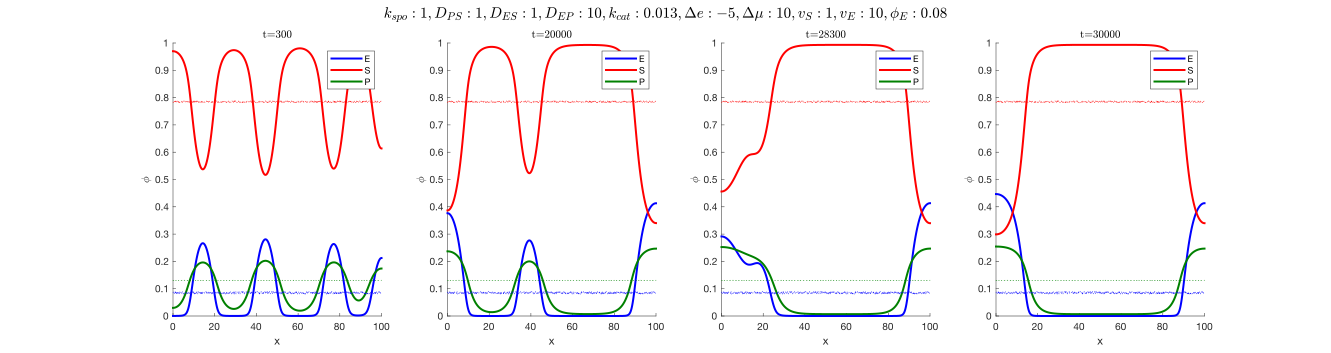
\includegraphics[width=8cm]{figures/high_enz.svg}
\end{figure}
\begin{figure}[b]
  \makebox[\textwidth][c]{\includesvg[width=10in]{figures/high_enz.svg}}
  \makebox[\textwidth]{\parbox{1.35\textwidth}{\caption{Numerical simulation of the incompressible active mixture studied in this work, with the specified system parameters. The faint, dashed lines show the initial distribution of components and the bold lines show the components at the stated times (t=300, 20000, 28300 and 30000). The free cross mobilities were given by $M_{ij}=-D_{ij}\phi_i\phi_j$. The position lattice was made up of 1000 lattice sites.}}}
\end{figure}

Figure 2 shows the evolution of the same system as figure 1 except with a lower initial enzyme concentration $\phi_E^*=0.08 \rightarrow 0.05$. Similarly to the system with more enzyme, small perturbations in the initial enzyme distribution grew rapidly and ultimately the system separated into a dense and dilute region. For both values of $\phi_E^*$ the enzyme volume fraction in the dense region was observed to be very similar ($\phi_E^*\approx0.25$), with the system containing higher overall enzyme having a wider dense region. This naturally suggests an upper limit on the amount of enzyme which is when all the system is in the dense phase, however the stability condition was lower than this. It is expected that this lower critical value of $\phi_E^*$ is due to the non-zero transition width between the two phases, meaning that stability changes in the limit of only the dense phase and the transition region.

\begin{figure}[t]
  \makebox[\textwidth][c]{\includesvg[width=8in]{figures/low_enz.svg}}
  \makebox[\textwidth]{\parbox{1.35\textwidth}{\caption{Numerical simulation of the incompressible active mixture studied in this work, with the specified system parameters. The faint, dashed lines show the initial distribution of components and the bold lines show the components at the stated times (t=300, 9500, and 10300). The free cross mobilities were given by $M_{ij}=-D_{ij}\phi_i\phi_j$. The position lattice was made up of 1000 lattice sites. Note the the lower enzyme volume fraction in the system, $\phi_E^*$=0.05.}}}
  \label{fig:low_enz}
\end{figure}

The linear stability analysis around the homogeneous steady state does not help understand the long-time dense and dilute phase separation. One approach that might provide further insight into these two regions would be to construct a quasi-free energy from assuming fast reaction dynamics, in addition to the fast substrate and product diffusion. Assuming that the reaction terms occurred very quickly at all points such that $R=0$ everywhere, the value of $\phi_S(x)$ and $\phi_P(x)$ could be solved from $\phi_E(x)$ (using relationships from equations (\ref{sstar}) and (\ref{pstar})). This could be substituted into equation (\ref{evoE}) which describes the evolution of the enzyme and used to try to construct a quasi-free energy that would give these dynamics and might identify the two phases.

\section{Further Work}

In development of this basic model we set all interaction parameters to zero, which allowed the subsequent investigation to discern the effects of the activity more clearly. Re-introducing these parameters is likely to simply make it harder or easier for the activity to induce this stability, depending on the signs of the interaction terms. However for the multi-component system, it is not obvious how different interaction terms (e.g. $\chi_{ES}$  or $\chi_{EP}$) may affect the overall stability of the homogeneous state and this would require further analysis. 

Another extension to this model would be to consider more complex reaction networks. Here we simply have one fuel driven, and one spontaneous reaction. A wide variety of behaviour can be seen in reaction networks, with a specific example being oscillatory behaviour. If this simple incompressible fluid contained more species we may see more complex behaviour, for example travelling waves or other kinds of oscillations, however this is speculative. The reaction dynamics could also be modified for non-trivial stoichiometry, with one particular example being $N \times \text{Monomers} \rightarrow \text{Polymer}$ and where $v_{Polymer} = N \times v_{Monomer}$ to maintain incompressibility. The analytic stability condition derived here could be done so in a general case consisting of only the $R_i$, $v_i$ and $M_{ij}$ terms and applied to other reactions.

Here, we considered only a noise free system with deterministic governing equations. The introduction of noise can often lead to additional behaviour, for example this might sustain multiple dense-dilute regions in the system. To add these terms back in, care must be taken to ensure the appropriate mobility symmetries and incompressibility conditions are respect. For example, simply adding in a noise term to $\textbf{J}_i$ as done in equation (\ref{modB2}) would break this and so a suggested scheme would be to introduce a term with the necessary mobility prefactors, for example  adding in a $\sum_i M_{ij}\zeta_j$ to the $i^{\text{th}}$ current, where $\zeta_j$ is a noise term.

\section{Outlook}

-Add interaction terms
-Couple to elastic terms
